\setsection{Améliorations notables : fausses alertes et outils de mesure}

	Comme nous l'avons vue précédemment (section 3) le problème de fusion de chaîne a amené à créer les \glspl{rainbow}. Mais il se peut aussi qu'il y ait collision entre la chaîne que nous générons et une des chaînes des tables. Lorsque ce cas arrive nous parlons de fausse alertes \cite{checkpoints}.
	De plus jusqu'à présent nous n'avons pas réellement présenté d'outils permettant de comparer les efficacités des différentes méthodes de \gls{TMTO}.

\setsubsection{Points de contrôles}

	Afin de vérifier que 2 chaînes ne fusionnent pas, il a été proposé par \cite{checkpoints} d'instaurer des points de contrôle. Pour ce faire, $\alpha_i$ positions sont fixées. Pour chaque chaîne, la fonction G est évaluée et la valeur est stockée, à chacune de ces positions. Lors de la génération de la chaîne $Y_1,Y_2,\ldots{},Y_s$ nous évaluons également les $G(Y_{\alpha_i+s-t})$. La moindre différence entre les points de contrôle de cette chaîne et celle de la table correspond à une fausse alerte.

	\bigskip

	les points de contrôle doivent être simple à évaluer et stocker, il est considéré que g sort les bits les moins significatifs. nous estimons selon la formule suivante la détection d'une fausse alerte :

	\begin{align*}
	pr\{g(x_{j,\alpha}) \neq g(y_{\alpha +s-t}) \mid x_{j,a} \neq y_{\alpha+s-t}\}=\frac{1}{2}(1-\frac{1}{2^{\mid k \mid}}) \approx \frac{1}{2}
	\end{align*}

\begin{samepage}
	Suite à l'introduction de ces points de contrôle, nous pouvons nous retrouver dans 2 cas :
	\bi
		\item soit le point de contrôle se trouve avant la fusion (figure de gauche ci-dessous), auquel cas nous pouvons détecter une fausse alerte avec une probabilité de $\frac{1}{2}$ comme vue ci-dessus
		\item soit le point de contrôle se trouve après la fusion (figure de droite ci-dessous)
	\ei
	\begin{figure}[H]
		\begin{minipage}{.5\textwidth}
			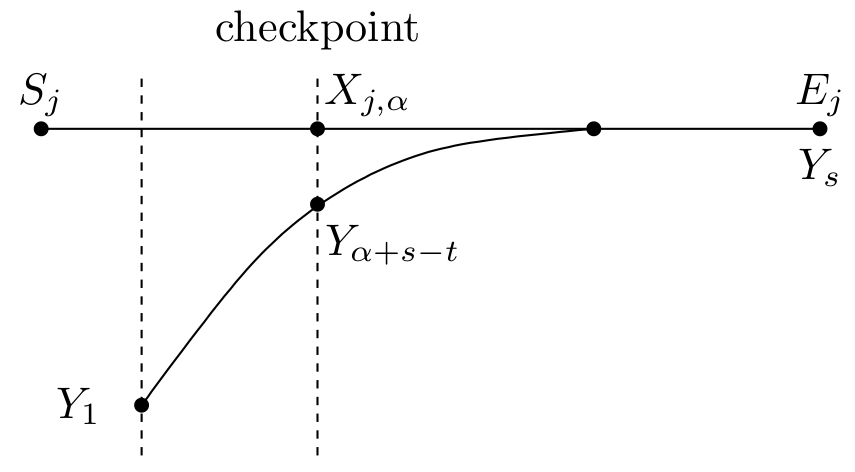
\includegraphics[width=0.9\linewidth]{other/FalseAlarmDetected.png}
			\captionof{figure}{Fausse alerte détectée}
		\end{minipage}
		\begin{minipage}{.5\textwidth}
			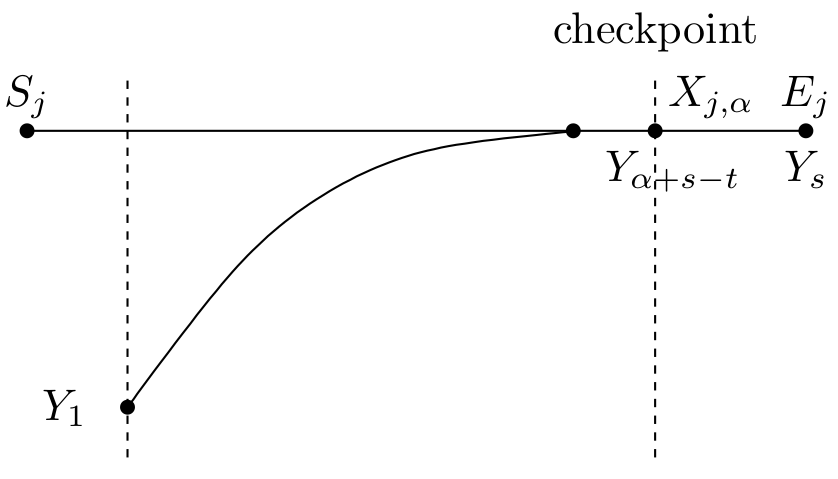
\includegraphics[width=0.9\linewidth]{other/FalseAlarmNotDetected.png}
			\captionof{figure}{Fausse alerte non détectée}
		\end{minipage}
	\end{figure}
\end{samepage}

\setsubsection{Tables parfaites}

	Cette notion de fusion et de points de contrôle introduit alors un nouveau concept les tables dites parfaites, des tables sans fusion. En effet comme l'équation de la courbe de compromis est de la forme $TM^2=\alpha *N^2$, afin de profiter au maximum du \gls{TMTO} il faut minimiser le coût mémoriel qui est élevé au carré. Et pour ce faire nous devons éviter de stocker de l'information redondante.

	\bigskip

	Pour créer une table de Hellman parfaite, il faut vérifier que chaque élément de la table soit distinct, ce qui est extrêmement coûteux à réaliser lors de la phase de pré-calcul. Cette vérification est nécessaire car une chaîne peut fusionner à n'importe quelle position d'une autre chaîne.

	\bigskip

	Afin de vérifier si une \gls{rainbow} est parfaite, il suffit de vérifier que chaque élément de fin de chaîne est distinct. Cette vérification est suffisante car la fonction de réduction change à chaque colonne.

	\bigskip

	De même, pour vérifier si une table de Hellman associé à la méthode des points distincts est parfaite, il suffit également de vérifier que chaque dernier élément est distinct. Cette vérification est suffisante car peu importe où commence la fusion dans tous les cas elle amènera au même point qui respecte le critère d'arrêt.

\setsubsection{Outils de comparaison}

	En connaissant les fonctions caractéristiques il est possible de tracer les graphiques temps-mémoire pour un taux de succès fixé. Ces graphiques montrent que le temps de calcul diminue avec le carré de la mémoire utilisée.

	\begin{align*}
		\label{simple}
		T=\frac{N^2}{M^2}\gamma(P)
	\end{align*}

	Où $\gamma(P)$ est facteur dépendant du taux de succès. Le cas optimal de P=86\% selon \cite{checkpoints} donne un facteur de $1$. Il est possible alors de retrouver le compromis typique proposé par Hellman \cite{ehellman}, $M=T=N^{\frac{2}{3}}$. La formule \ref{simple} permet de trouver un des paramètres optimaux, en se basant sur les 2 autres.

	\bigskip

	Afin de comparer l'efficacité des différentes méthodes de \gls{TMTO}, il est possible d'étudier l'évolution de $\gamma{P}$.

	Les tables classiques et DP peuvent aussi être caractérisées par le facteur $\gamma$. Dans cette étude, il a été choisi de générer les plus grosses tables parfaites possibles, et autant de tables que nécessaire pour atteindre un taux de succès P fixé. Les caractéristiques sont tracées en figure \ref{fig:TMTO_carac}, par ailleurs les sauts de la courbe de la méthode \gls{rainbow} correspondent à la nécessité d'une table supplémentaire.

	\begin{figure}[H]
		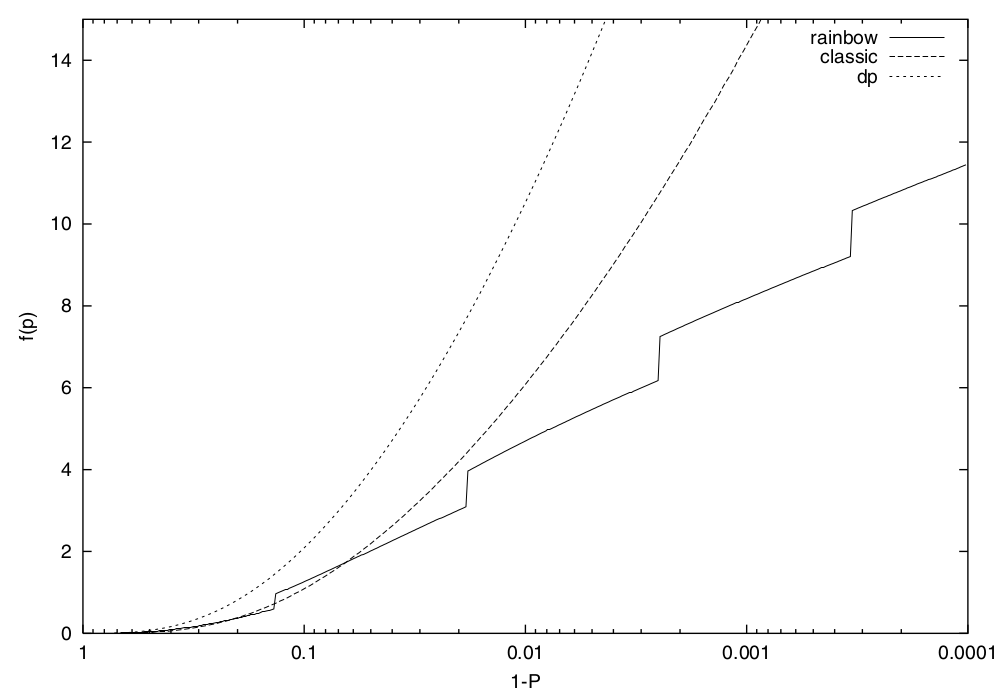
\includegraphics[scale=0.25]{other/graph_gamma_P.png}
		\captionof{figure}{Graphique Temps-Mémoire pour les tables classiques, arc-en-ciel et DP}
		\label{fig:TMTO_carac}
	\end{figure}

	La théorie et l'expérience montrent qu'à partir d'un taux de succès de 80\%, les \glspl{rainbow} proposent le meilleur compromis. En dessous de ce taux, il semblerait que les tables classiques soient un peu meilleures. Mais elles conservent un coût de temps de calcul plus élevé, lié à la nécessité de t fois plus de boucles lors de la recherche dans les tables.

\setsubsection{Conclusion}

	La méthode des points de contrôle est une évolution extrêmement intéressante qui permet de limiter le coût en temps de calcul, de plus elle peut s'appliquer à toutes les méthodes de \gls{TMTO}.

	\bigskip

	Nous avons également vu plus en détail la méthode de comparaison entre les différentes méthodes de \gls{TMTO}.

\endinput{}
